%---------------------------------------------------------------------------------------------------
%		cloud.tex
%
%	This file contains the sections of the document that describe the cloud computing.
%
%	Author: Andrea Meneghinello
% Version: 0.1
%	Table of changes:
%		15/03/2016 -> document definition
%---------------------------------------------------------------------------------------------------
\section{Cloud Computing}
\label{sec:background-cloudComputing}
Cloud computing provides shared resources and data to devices on-demand; providers commonly offer a 
``\keyword{\glossarySng{pay-per-use}}'' model to pay used resources. Hence the pay-per-use model
in \acs{it} is becoming available to the market. It has been proved that it is an effective way to
reduce \acs{it} costs without sacrificing software quality. Consequently the demand for highly
responsive, reactive and cheap \ac{saas}, made by end-users and companies, is increasing (as shown
in Figure \ref{img:background-cloudComputing-saasInterest}).

%TODO -> controllare se inserire una reference in "It has been proved"
 
\begin{figure}
	\centering{}
 	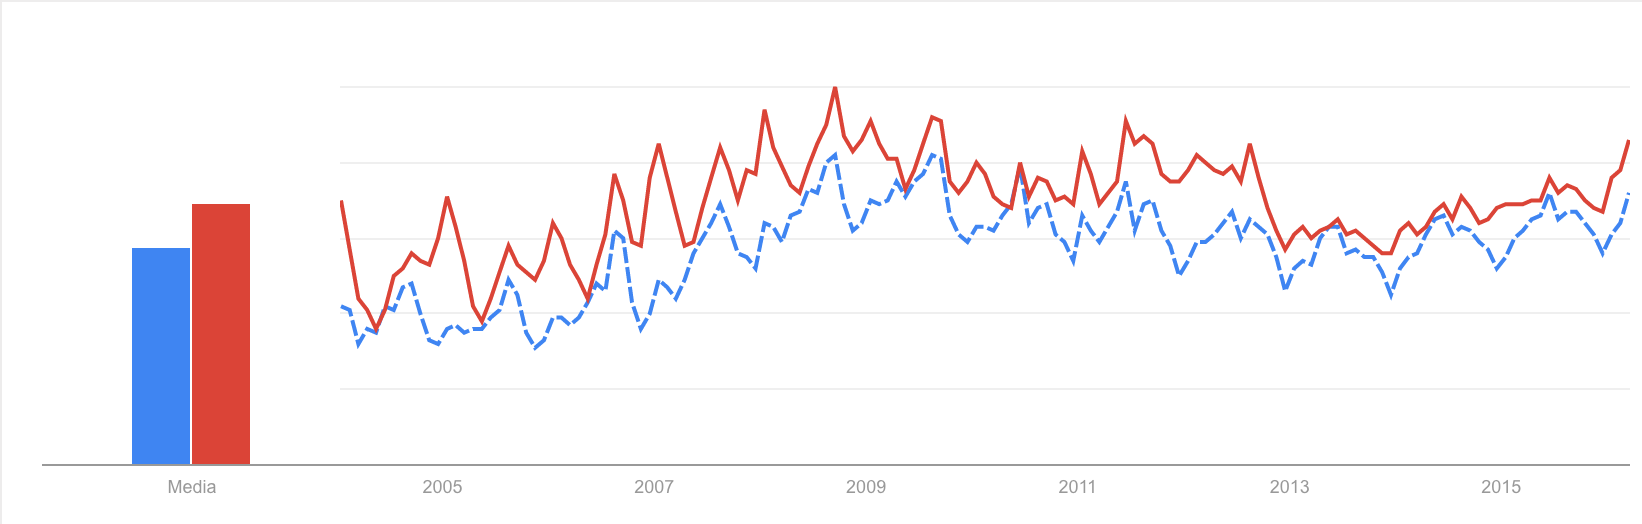
\includegraphics[width=0.75\textwidth]{chapters/background/images/saas-interest.png}
 	\caption[Trends in searching ``\acs{saas}'' on Google]{\acf{saas} and its acronym (\acs{saas})
 		terms search since 2004 in Google's investigation made all over the world. In red we can see
 		results about ``\acs{saas}'' term search instead in blue we have the ``\acf{saas}'' one. 
 		(\footnotesize{source	Google Trends}\normalsize{)}}
 	\label{img:background-cloudComputing-saasInterest}
\end{figure}

Cloud computing helps also software-houses, providing them \keyword{ready-to-use work environments}.
This solution makes software-houses save both money and time because developers do not waste time in 
building the work environments on their own. In addiction those work environments are \keyword{elastic},
hence they can build and deploy their application and make them ubiquitous. Therefore the demand for
this particular kind of cloud platform is increasing, as shown in Figure
\ref{img:background-cloudComputing-paasInterest}.

\begin{figure}
	\centering{}
	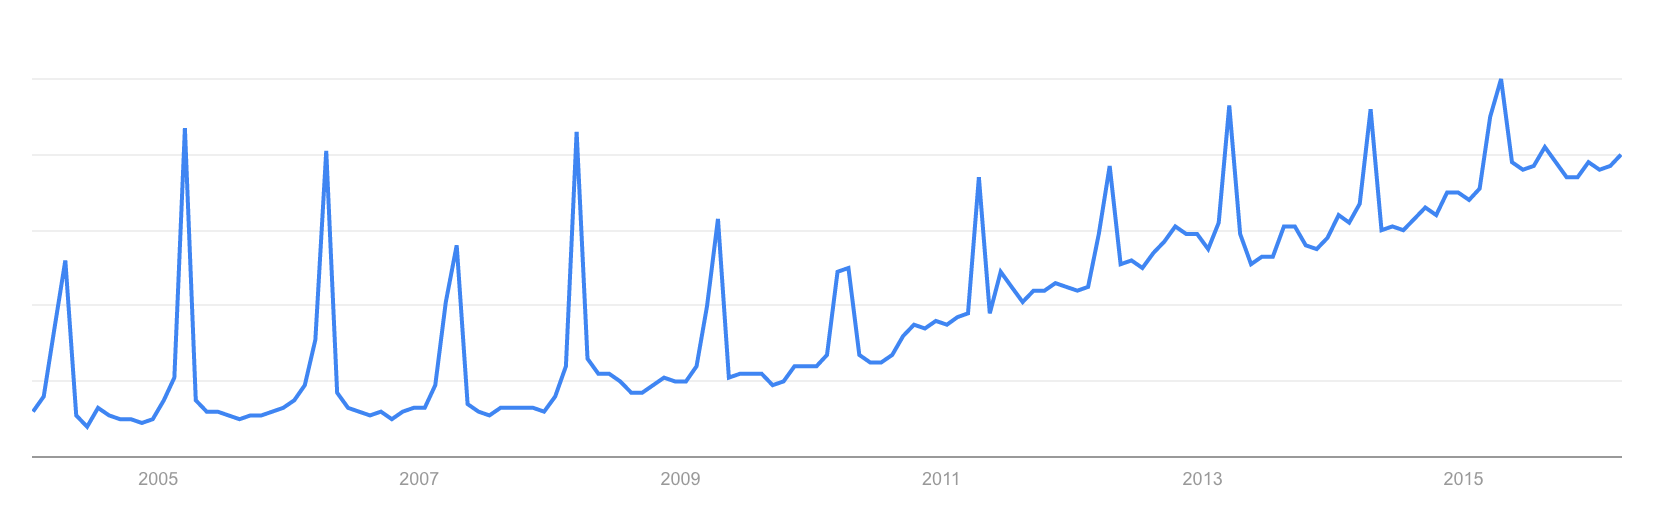
\includegraphics[width=0.75\textwidth]{chapters/background/images/paas-interest.png}
	\caption[Trends in searching ``\acs{paas}'' on Google]{\acf{paas} terms search since 2004 in Google's
		investigation made all over the world. (\footnotesize{source	Google Trends}\normalsize{)}}
	\label{img:background-cloudComputing-paasInterest}
\end{figure}

To make their software exploit the elasticity offered by cloud environments, software-houses need to redesign
them using appropriate architectural patterns. Before discussing about those patterns, it is necessary to do a
brief digression about what cloud computing really is and why in the nearly future many more companies and
software-house will start a migration to it.

The most comprehensive definition of what cloud computing is comes from \ac{nist} in \cite{nistCloudComputing}:

\begin{center}
	\begin{quote}
		\textit{``a model for enabling ubiquitous, convenient, on-demand network access
			to a shared pool of configurable computing resources that can be rapidly provisioned and released
			with minimal management effort or \acf{sp} interaction."}
	\end{quote}
\end{center}

In following Sections we will show, in details, the benefits of its adoption by presenting its main
characteristics.

\subsection*{Moving from platform ownership to platform management}
\label{sec:background-cloudComputing-capexOpex}
When companies decide to design, and consequently build, a new software service they have to plan how
many resources (compute capacity, storage and networking) making available in order to respect the defined
\ac{sla}. Developers have to build, over the provisioned resources, the working environment to build
and support the application.

This leads to predict the worst possible cases and to invest in resources that permit to cope this
situation as well as find a business grow model that maintains enough availability without weighing
too much on the investments. Even if this prediction is able to detect the worst cases it imposes
large capital investments and heavy fixed costs on firms, which lead to redundant expenditures and
high level of overcapacity, both in term of technology and in term of qualified personnel in its
management. The cited business model is known with the name of \keyword{\ac{capex}}.

Opposite to the \ac{capex} business model there is the \keyword{\ac{opex}}. This is more flexible
because it does not require to invest in capital ownership (hardware and time to build the work
environment) but instead in renting both the desired amount of resources and the ready-to-use work
environments and simply release them when they are no more necessary. This model, if correctly applied,
permits a cost reduction; Figure \ref{img:background-capexOpex-model} shows a chart which compares
both models. We can also see that there will be a moment (in the adoption of \ac{capex} one) on which
there is a lack in the available resources leading to a decline of the service and to a possible \ac{sla}
violation.

\begin{figure}
	\centering{}
	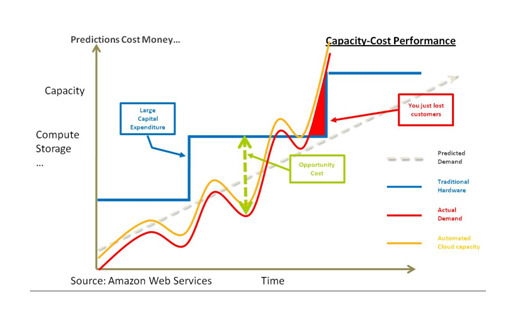
\includegraphics[width=0.9\textwidth]{chapters/background/images/capex-opex.png}
	\caption[Comparison between \acs{capex} and \acs{opex} business models]{Comparison of \acf{capex}
		and \acf{opex} business models.}
	\label{img:background-capexOpex-model}
\end{figure}

We can observe these two different business models also in two real case scenarios \cite{netflixZynga}
that involve two well known software houses, in the world of mobile/social-network games and the other
in video content sharing: they are \textit{Zynga} and \textit{Netflix}. 

The most famous product of Zynga is \textit{Farmville}. It was released in 2009 and became, in a very
short period, very popular between Facebook users (it reached 10 million of active users in less than
6 weeks). Initially the service was hosted inside the Amazon infrastructure but two years later his
\acs{ceo}, Frank D. Gibeau, decided to invest \textdollar{}100 million to build a proprietary data-centre
to host the service assuming to obtain a long term cost reduction. In Figure
\ref{img:background-capexOpex-zyngaCase} we can see the trend of \ac{mau} of Farmville application
in the months that follow the opening of new data-centre. It is possible to observe that \ac{mau} reached
its peak in 2012 (when the new centre became operative) but in the following two years this value had
been divided by three (as the new infrastructure demanded), leading to consistent economic losses.
Thus the society has decided to return basing its service on the Amazon Infrastructure.

\begin{figure}
	\centering{}
	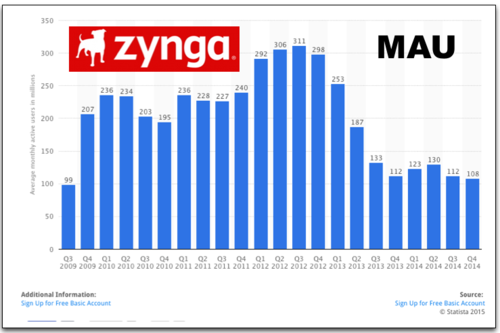
\includegraphics[width=0.6\textwidth]{chapters/background/images/zynga-case.png}
	\caption[\acs{mau} of Farmville application after 2012]{\acf{mau} of the Farmville application from
		2012 when company decide to invest in a proprietary data-centre. We can observe that after two
		years the users' demand is divided by three as the infrastructure demand \cite{netflixZynga}.}
	\label{img:background-capexOpex-zyngaCase}
\end{figure}

Netflix, born in 1997 with a rent \acs{dvd} service, started a new \ac{vod} business in 2007 and, as
in the case of Zynga, chose to base its new business on the Amazon infrastructure. The most relevant
difference is that Netflix never chose to change its infrastructure supplier when it saw that his
business was starting to succeed. This choice allowed Netflix to become the major \ac{vod} competitor.

\subsection*{Cloud Computing key characteristics}
\label{sec:background-cloudComputing-characteristics}
Taking as a reference the \ac{nist} definition of cloud computing \cite{nistCloudComputing}, a pool of resources
must offer the following characteristics (shown in Figure \ref{img:background-cloudComputing-characteristics})
to the end-users to be considered a cloud environment:

\begin{itemize}
	\item{\keyword{on-demand self-service}: refers to way on which people can procure resources, specifically
		they should be made available to users on-demand with automatic procedures;}
	\item{\keyword{broad network access}: refers to the way on which people can get them; a cloud provider
		must not restrict the access to them by imposing the use of a particular technology;}
	\item{\keyword{resource pooling}: refers on the way on which the cloud provider makes them available to
		customers; it must make them accessible as a single and compact set of resources even if the are
		distributed on many servers inside the data-centre;}
	\item{\keyword{rapid elasticity}: refers on the way on which resources can be provisioned and released
		to maintain the software highly available while keeping the monthly/hour\footnote{Usually we have a
		monthly rent in case of adoption of \acs{paas} cloud model, instead we have a hour rent if we adopt
		a \acs{iaas} cloud model. We illustrate the difference in following sections.} rent as low as possible;}
	\item{\keyword{measured service}: refers on the way on which both the end-user and the cloud provider
		can measure the resource consumption. This is fundamental for final users to know the total amount of
		the rent and for cloud provider to keep under control resource consumption and scale them only when
		it is really necessary.}
\end{itemize}

\begin{figure}
	\centering{}
	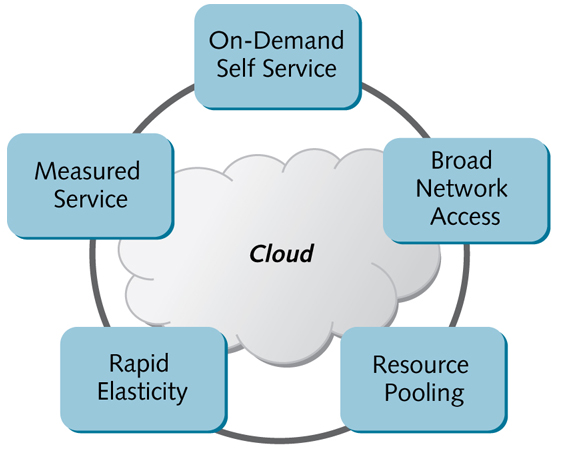
\includegraphics[width=0.5\textwidth]{chapters/background/images/cloud-characteristics.png}
	\caption[Key characteristics of cloud computing]{An overview of the five characteristics that makes a
		pool of shared resources a cloud computing environment \cite{cloudCharacteristics}.}
	\label{img:background-cloudComputing-characteristics}
\end{figure}

\subsection*{Available service models}
\label{sec:background-cloudComputing-cloudServiceModels}
Nowadays cloud computing makes available many service models (shown in Figure
\ref{img:background-cloudComputing-serviceModels}):

\begin{itemize}
	\item{\keyword{\acf{saas}}: the capability provided to the end-user is to use the provider's
		applications running on a \glossarySng{cloudInfrastructure}. Programs are accessible from various
		client devices through either a thin interface, such as a web browser (e.g. web-based e-mail),
		or a program interface. The user does not manage or control the underlying cloud infrastructure
		including network, servers, operating systems, storage, or even individual application capabilities,
		with possible exception of limited user specific application's configuration settings;}
	\item{\keyword{\acf{paas}/\ac{caas}}: the capability provided to the end-user is to deploy onto the cloud
		infrastructure user-created or acquired applications created using programming languages,
		libraries, services and tools supported by the provider.\footnote{This capability does not preclude
		use of compatible tools like other sources.} The user does not manage or control the underlying
		cloud Infrastructure including network, servers, operating systems or storage, but has control
		over the deployed applications and possibly configuration settings for the application-hosting
		environment;}
	\item{\keyword{\acf{iaas}}: the capability provided to the end-user is to provision processing, storage,
		network and other fundamental computing resources where the consumer is able to deploy and run
		arbitrary software, which can include \acs{os} and applications. The final user does not
		manage the underlying cloud infrastructure but has control over operating systems, storage, and
		deployed applications; and possibly a limited control of selected networking components (such as
		network firewall).}
\end{itemize}

To help to understand how these three components are related together, Randy Bias \cite{differenceIaasPaas}
create this transportation analogy:

\begin{quote}
	``By itself, infrastructure is not useful. It just sits there waiting for someone to make it productive in
	solving a particular problem. Imagine the Interstate transportation system in the \acs{us} Even with all
	these roads built, they would not be useful without cars and trucks to transport people and goods. In this
	analogy, the roads are the infrastructure and the cars and trucks are the platform that sits on top of the
	infrastructure and transports the people and goods. These goods and people might be considered the software
	and information in the technical realm''.
\end{quote}

\begin{figure}
	\centering{}
	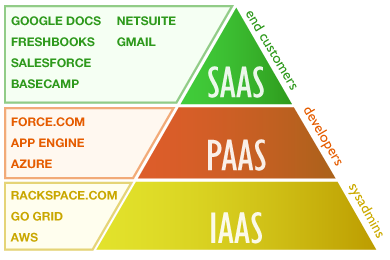
\includegraphics[width=0.55\textwidth]{chapters/background/images/cloud-service-models.png}
	\caption[Available service models in cloud computing]{An overview of available cloud service models. On the
		left we can observe example of ``environments'' that uses the specified models, while on the right we
		have the people interested for that specific models \cite{cloudServiceModels}.}
	\label{img:background-cloudComputing-serviceModels}
\end{figure}

\subsection*{Available deployment models}
\label{sec:background-cloudComputing-cloudDepoymentModels}
Cloud Computing can assume different forms:

\begin{itemize}
	\item{\keyword{Private Cloud}: the cloud infrastructure is provisioned and used by a single organization
		comprising multiple customers (e.g. business units). It may be owned, managed and operated by the
		organization, a third party or some combination of them and it may exist on or off premises;}
	\item{\keyword{Community Cloud}: the cloud infrastructure is provisioned for exclusive use by a specific
		community of users from organizations that have shared concerns (e.g. mission, security requirements,
		policy, and compliance considerations). It may be owned, managed and operated by one or more of
		the organizations in the community, a third party or some combination of them, and it may exist on
		or off premises;}
	\item{\keyword{Public Cloud}: the cloud infrastructure is provisioned for open use by the general
		public. It may be owned, managed and operated by a business, academic, government organization or
		some combination of them, and it may exist on or off premises;}
	\item{\keyword{Hybrid Cloud}: the cloud infrastructure is a composition of two or more distinct
		cloud infrastructures (private, community or public) that remain unique entities, but are bound
		together by standardized or proprietary technology that enables data and application portability
		(e.g. cloud bursting for load balancing between clouds).}
\end{itemize}

\subsection*{Isolation and resource control}
\label{sec:background-cloudComputing-isolationResource}
With the adoption of cloud computing, software-houses have isolation between hardware management and the software
development that makes possible to separate the work of hardware engineers and software developers.
Now it is possible to maintain the hardware updated without worrying about the software. For example Amazon
System Engineers can decide to upgrade the storage hardware from the magnetic to solid state technology without
informing software-houses or users, that have applications deployed on it. On the other hand software-houses
and users do not need to alter and/or redeploy software after the change occurred. Often these changes are
transparent to the final users. 

However the introduction of cloud computing introduces a series of new problems that software developers must
master to develop high productive software. One critical issue that occurred when companies has began to use cloud 
computing is that they started to share a common base: the hardware on which the software executes.

\keyword{Isolation} and \keyword{resource control} have become two critical requirements when we are co-locating
applications of different companies in the same cloud computing environment. Isolation refers to the requirement
that execution of one software must not affect the execution of another one in the same system. Resource control
instead refers to the ability to constrain software execution to a specific set of resources.

In cloud settings, while performance isolation is desirable, it is often secondary to functional and security
isolation wherein one software cannot learn anything or affect the correctness of another one. Memory capacity
and compute capability are two levers in resource control through which a software is constrained to consume
no more than a certain amount of memory capacity and execute no more than a certain number of cores.